\documentclass[fontsize=11pt]{jlreq}
\usepackage{subfiles}
\usepackage{amsmath, amssymb, braket} % AMSの数式
\usepackage{lmodern} % 美文書入門 p.74 5.2数式用のフォント
\usepackage{graphicx,color} % https://texwiki.texjp.org/?hyperref
\usepackage{subcaption} % figureなどのキャプション
\usepackage{bm} % bold math
\usepackage{quantikz} % 量子回路図
\usepackage[version=4]{mhchem} % 化学式
\usepackage[backend=biber, style=numeric, maxnames=5, doi=false, url=true, eprint=true]{biblatex}
\addbibresource{quantum.bib}
\makeatletter
\let\mkbibemph=\mkbibitalic
\let\blx@imc@mkbibemph=\blx@imc@mkbibitalic
\makeatother
\setlength{\biblabelsep}{0.5em}

%\usepackage{pdfx}  % side-effect: hyperrefの設定もされる
\usepackage{hyperref} % リンクの埋め込み、pdfファイルの目次の生成
\hypersetup{
    colorlinks=true,
    linkcolor=blue,
    urlcolor=cyan,
    pdftitle={Quantum Circuit for First Quantization Hamiltonian Simulation Handling Coulomb Potential Pole},
    pdfauthor={Hideo Takahashi},
    pdfsubject={Research Paper},
    pdfkeywords={Quantum Computer, First Quantization, ab initio, Simulator, Coulomb Potential, Quantum Chemistry},
    bookmarksnumbered=true,
    bookmarksopen=true
}
\usepackage{paper2025}

\begin{document}
\title{フル量子回路による1,2次元水素原子モデルの\\
時間発展シミュレーションとその誤差解析\\
補助資料 (Supplimentary Material)}
\section{誤差を最小にするシミュレーションパラメタの決定方法の詳細}
\label{smsec:parameter-selection-for-minimum-error-analysis-details}

長い期間に渡って時間発展をした時の誤差評価。
\begin{figure}[ht]
    \centering
    \begin{subfigure}{0.45\columnwidth}
        \centering
        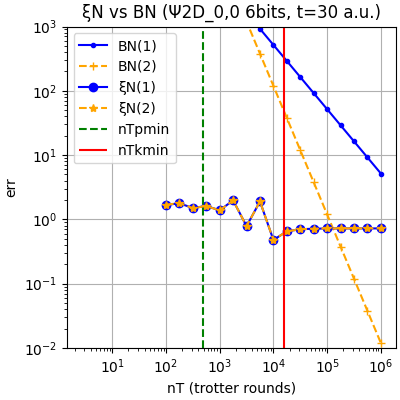
\includegraphics[width=1\columnwidth]{paper2025_figs/sdt_error/trotter_err_n0_m0_6b_t30.png}
        \caption{$\PsiTwoD_{0,0}, \nb=6, t=30.0$}
        \label{subfig:trotter-error-2d-0-0-6b-t30}
    \end{subfigure}
    \begin{subfigure}{0.45\columnwidth}
        \centering
        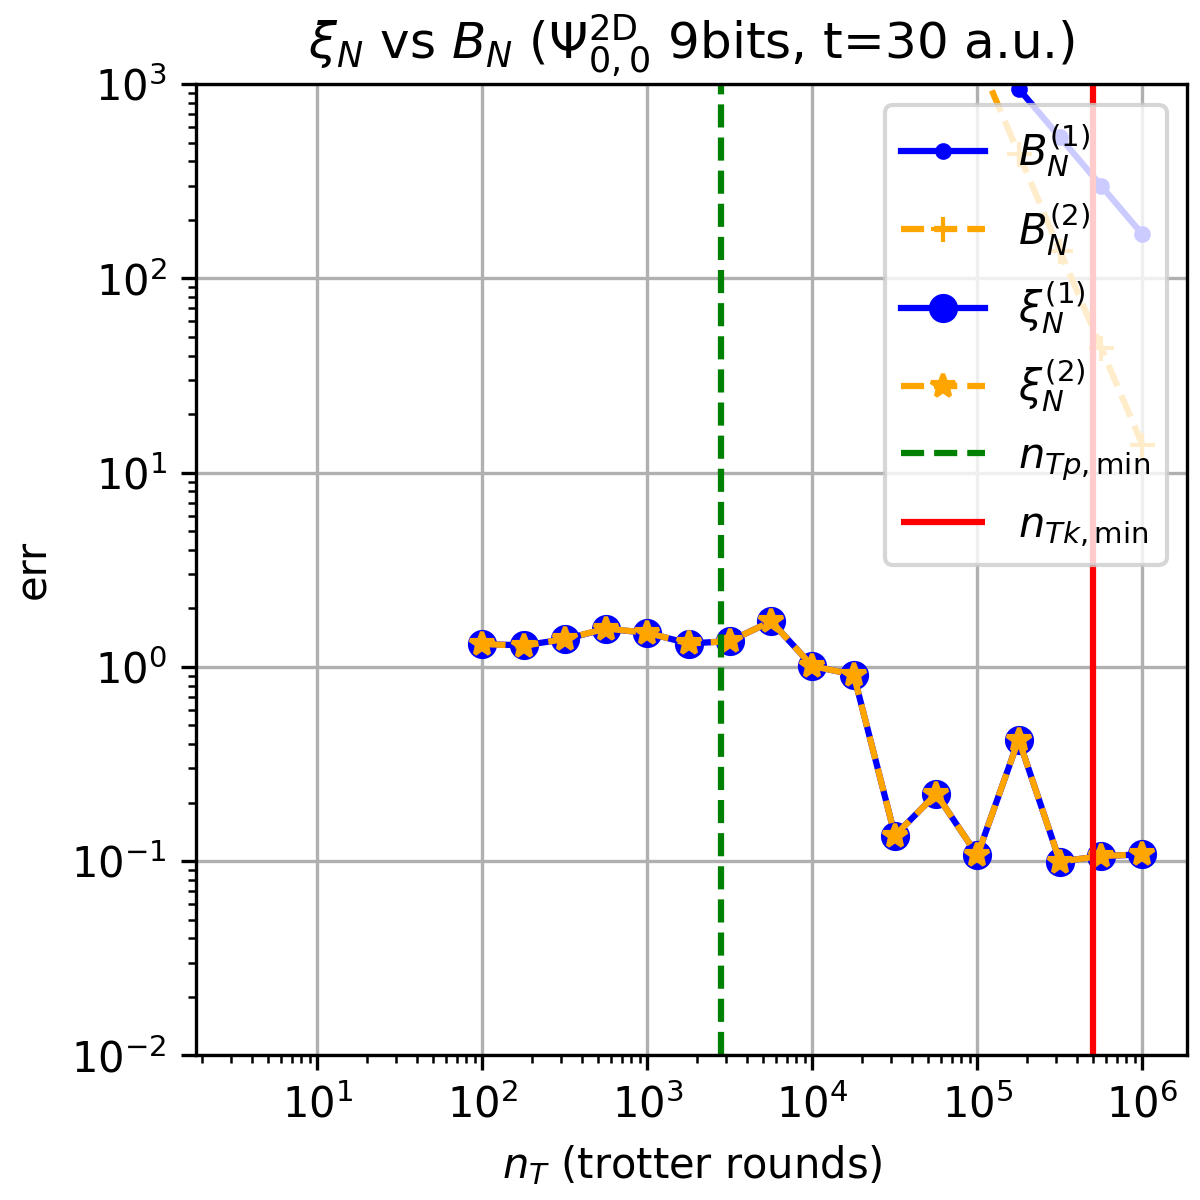
\includegraphics[width=1\columnwidth]{paper2025_figs/sdt_error/trotter_err_n0_m0_9b_t30.png}
        \caption{$\PsiTwoD_{0,0}, \nb=9, t=30.0$}
        \label{subfig:trotter-error-2d-0-0-9b-t30}
    \end{subfigure}

    \begin{subfigure}{0.45\columnwidth}
        \centering
        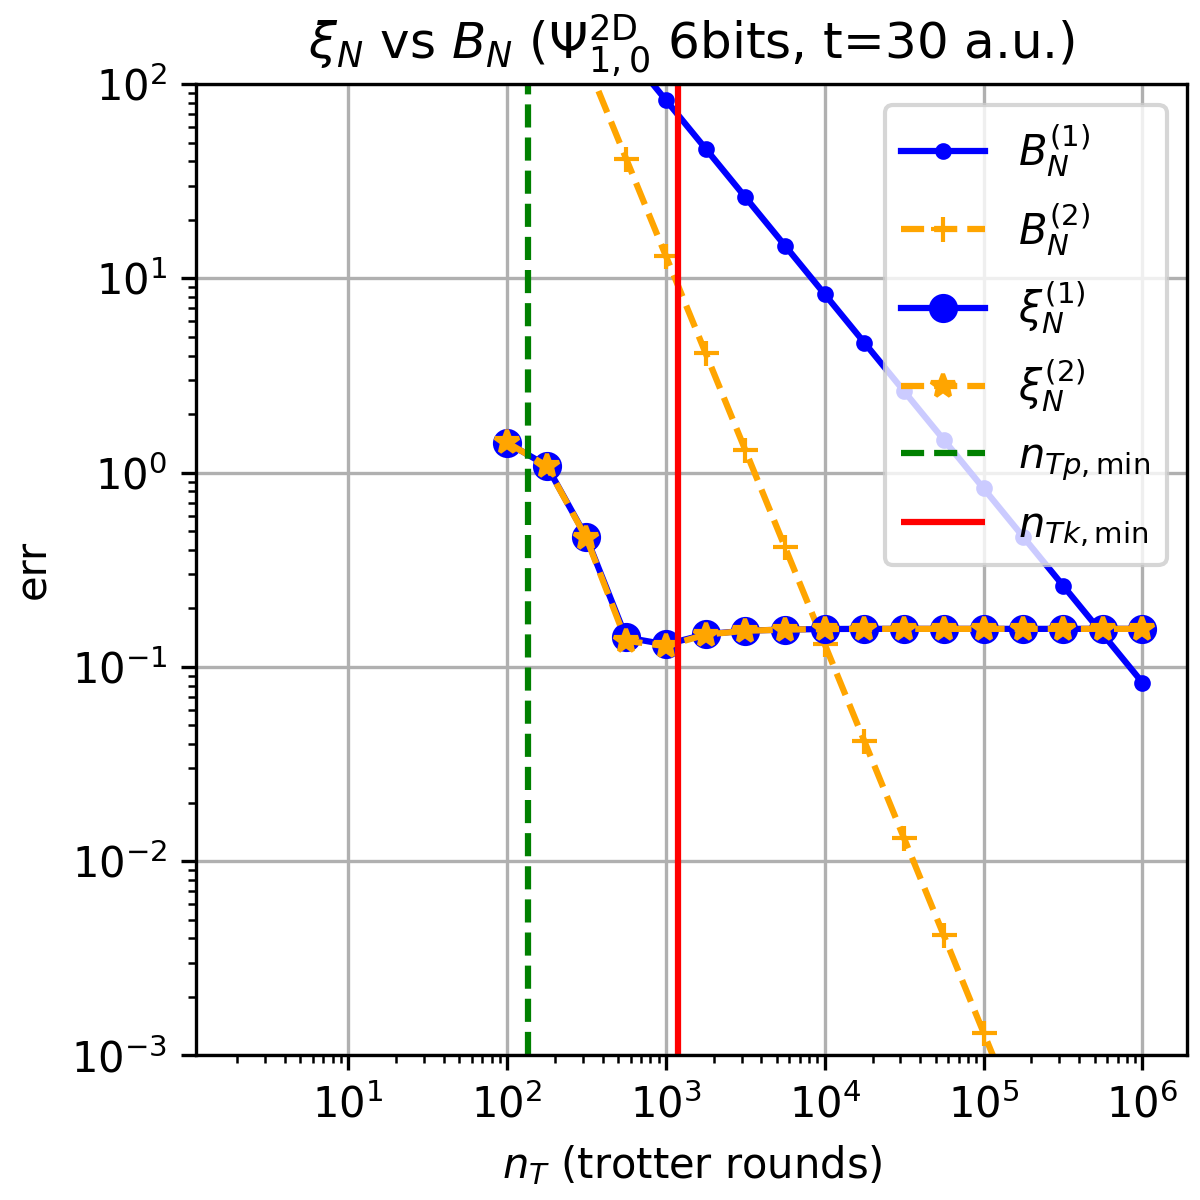
\includegraphics[width=1\columnwidth]{paper2025_figs/sdt_error/trotter_err_n1_m0_6b_t30.png}
        \caption{$\PsiTwoD_{1,0}, \nb=6, t=30.0$}
        \label{subfig:trotter-error-2d-1-0-6b-t30}
    \end{subfigure}
    \begin{subfigure}{0.45\columnwidth}
        \centering
        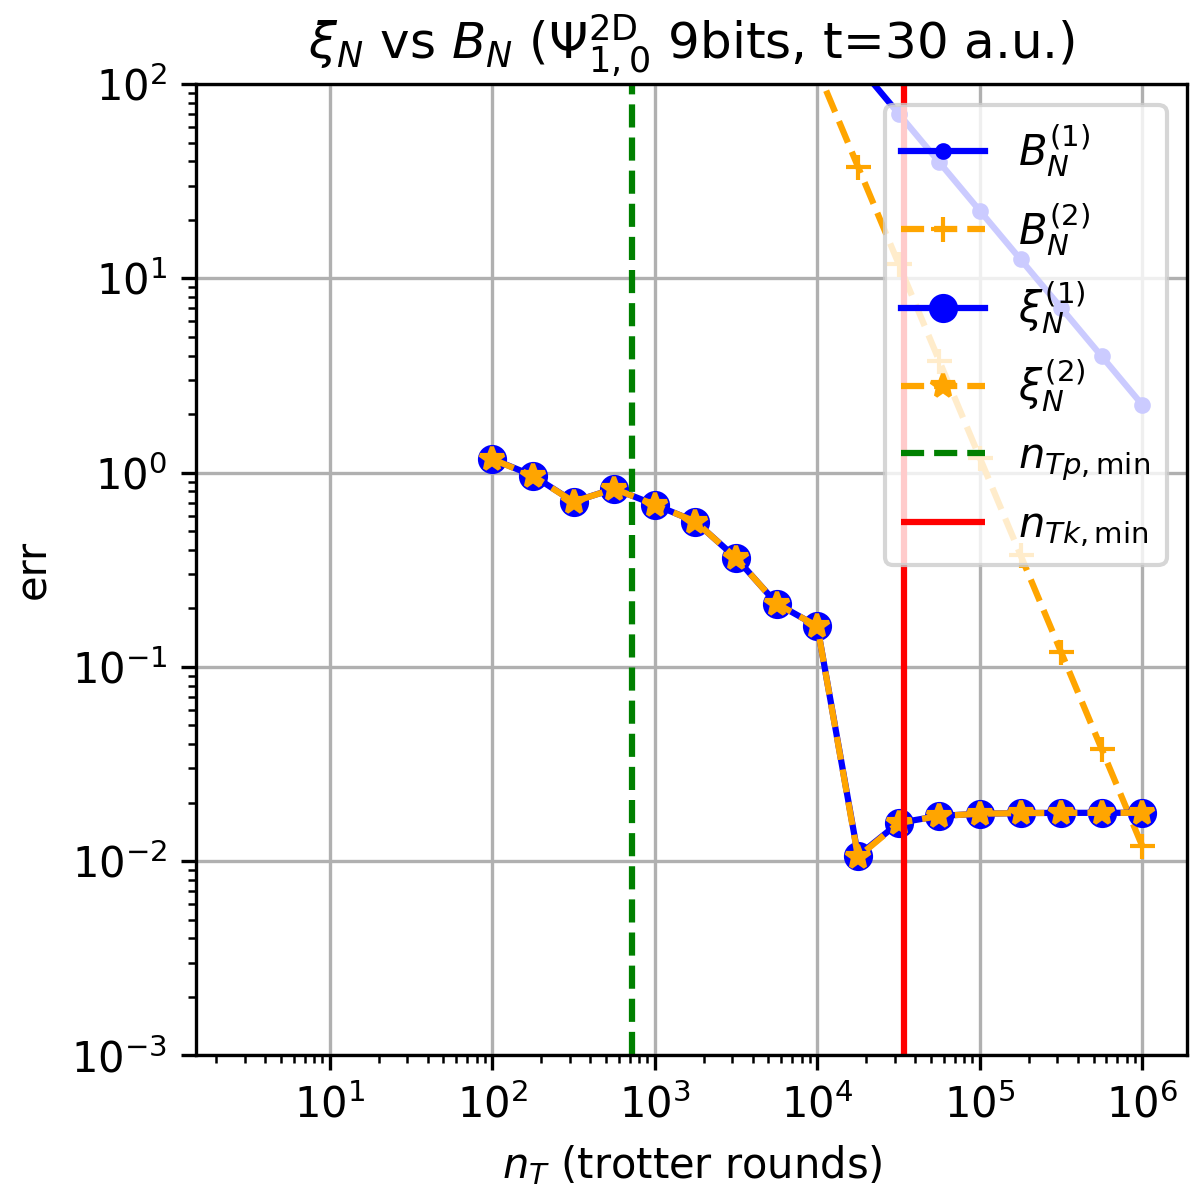
\includegraphics[width=1\columnwidth]{paper2025_figs/sdt_error/trotter_err_n1_m0_9b_t30.png}
        \caption{$\PsiTwoD_{1,0}, \nb=9, t=30.0$}
        \label{subfig:trotter-error-2d-1-0-9b-t30}
    \end{subfigure}

    \caption{時間発展期間$t=30.0$ での分割数$\nT$に対する誤差の上限 $\BN{\gamma}$ と観測値 $\xiN{\gamma}$}
    \label{fig:trotter-error-t30-part1}
\end{figure}

\begin{figure}[ht]
    \centering
    \begin{subfigure}{0.45\columnwidth}
        \centering
        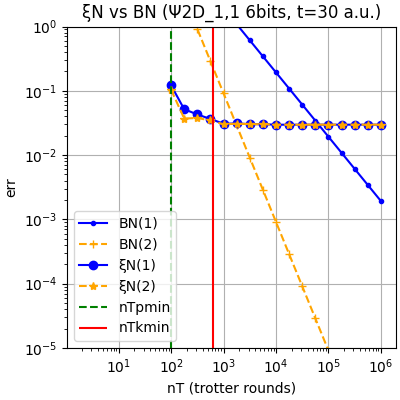
\includegraphics[width=1\columnwidth]{paper2025_figs/sdt_error/trotter_err_n1_m1_6b_t30.png}
        \caption{$\PsiTwoD_{1,1}, \nb=6, t=30.0$}
        \label{subfig:trotter-error-2d-1-1-6b-t30}
    \end{subfigure}
    \begin{subfigure}{0.45\columnwidth}
        \centering
        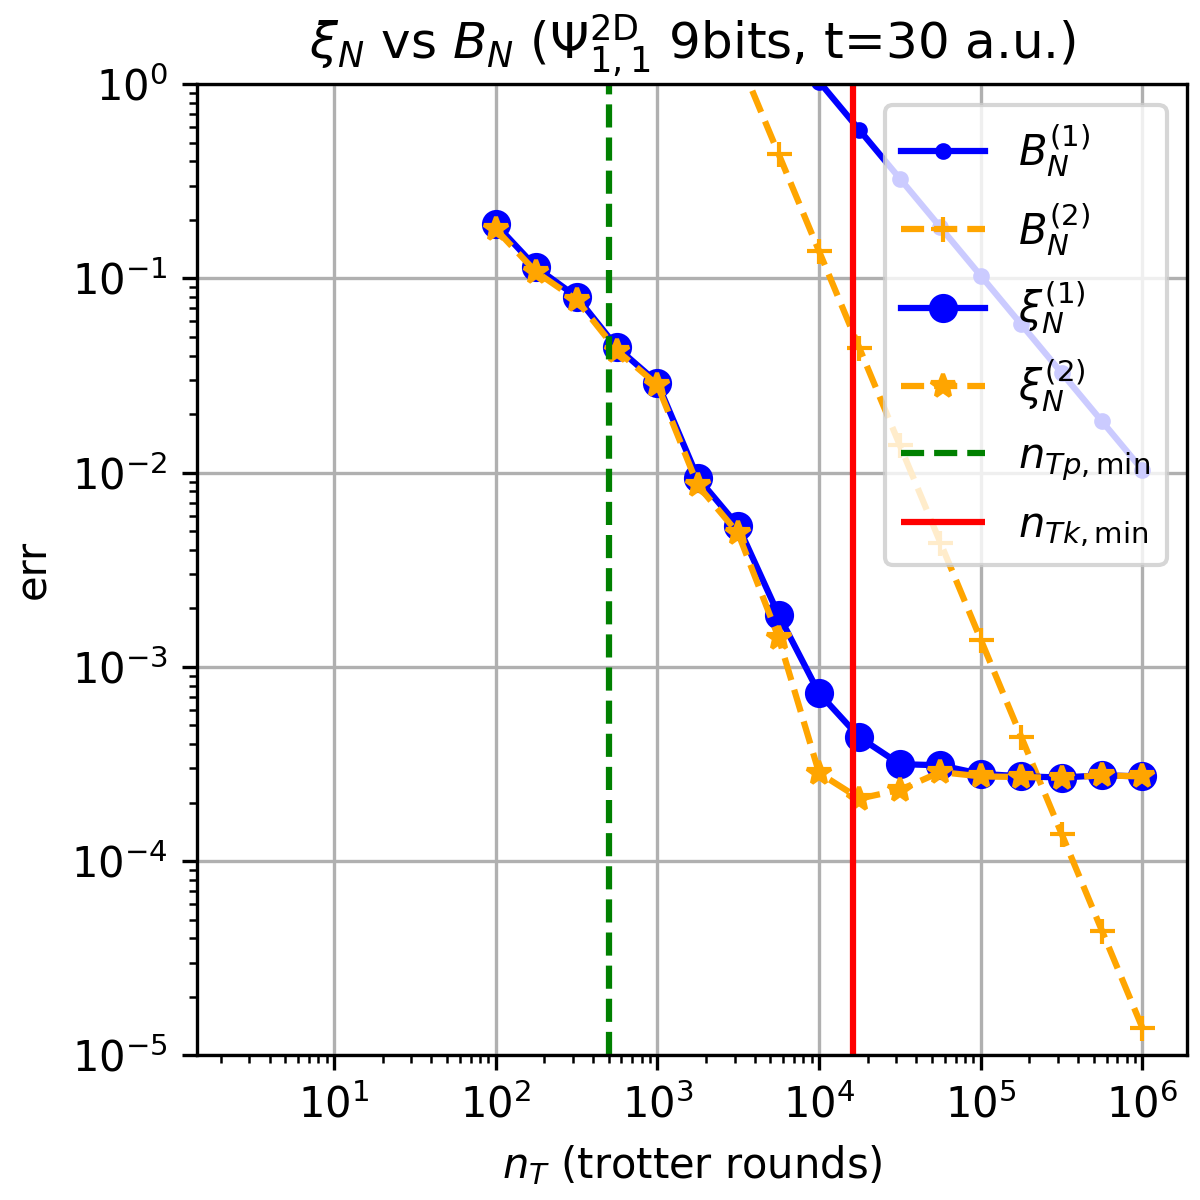
\includegraphics[width=1\columnwidth]{paper2025_figs/sdt_error/trotter_err_n1_m1_9b_t30.png}
        \caption{$\PsiTwoD_{1,1}, \nb=9, t=30.0$}  
        \label{subfig:trotter-error-2d-1-1-9b-t30}
    \end{subfigure}

    \caption{時間発展期間$t=30.0$ での分割数$\nT$に対する誤差の上限 $\BN{\gamma}$ と観測値 $\xiN{\gamma}$（つづき）}
    \label{fig:trotter-error-t30-part2}
\end{figure}

\end{document}
